\documentclass[../main.tex]{subfiles}
\begin{document}

\chapter{Introduction to M-Files }
\addcontentsline{toc}{section}{Chapter 3:Introduction to M-Files}

\section{WHAT ARE M-FILES?}

Up to now, all of our interactions with MATLAB have been directly through the command window. As we begin to work with more complicated algorithms, it will be preferable to develop standalone programs that can be separately stored and saved into files that can always be called on (by their name) in any MATLAB session. The vehicle for storing such a program in MATLAB is the so-called Mfile. M-files are programs that are plain-text (ASCII) files written with any word processing program (e.g., Notepad or MS Word) and are called M-files because they will always be stored with the extension $<filename>.m$\footnote{ It is recommended that you use the default MATLAB M-file editor gotten from the "File" menu (on 
the top left of the command window) and selecting "New"-> "M-File." This editor is designed 
precisely for writing M-files and contains many features that are helpful in formatting and debugging. 
Some popular word processing programs (notably MS Word) will automatically attach a certain 
extension (e.g., ".doc") at the end of any filename you save a document as and it can be difficult to 
prevent such things. On a Windows/DOS-based PC, one way to change an M-file that you have 
created in this way to have the needed ".m" extension is to open the DOS command window, change to 
the directory you have stored your M-file in, and rename the file using the DOS command ren 
$<filename>.m.doc <filename>.m$ (the format is: $ren <oldfilename>.oldextensio n <newfilename>.newextension$). } As you begin to use MATLAB more seriously, you will start to amass your own library of M-files (some of these you will have written and others you may have gotten from other sources such as the Internet) and you will need to store them in various places (e.g., certain folders on your own computer, or also on your portable disk for when you do work on another computer). If you wish to make use of (i.e., "call on") some of your M-files during a particular MATLAB session from the command window, you will need to make sure that MATLAB knows where to look for your M-files. This is done by including all possible directories where you have stored M-files in MATLAB's path.\footnote{Upon installation, MATLAB sets up the path to include a folder "Work" in its directory, which is the 
default location for storing M-files. To add other directories to your path, simply select "Set Path" 
from the "File Menu" and add on the desired path. If you are using a networked computer, you may 
need to consult with the system administrator on this. }

\textbf{EXAMPLE 3.1:} Here is a simple script which assumes that numbers $x 0, y 0$, and $r>0$ have been stored in the workspace (before the script is invoked) and that will graph the circle with center $(x 0, y 0)$ and radius $r$.

\begin{figure}[H]
\centering
\begin{boxedverbatim}
t= 0:.001:2*pi;
x = x0 + r * cos(t);
y = y0 + r *sin(t);
plot(x,y)
axis(`equal')
\end{boxedverbatim}
\end{figure}

If the above lines are simply typed as is into a text file and saved as, say, circdrw. $m$ into some directory in the path, then at any time later on, if we wish to get MATLAB to draw a circle of radius 2 and center $(5,-2)$, we could simply enter the following in the command window:

\begin{verbatim}
>> r=2; x0=5; y0= -2;
>>circdrw 

\end{verbatim}

and voilà! the graphic window pops up with the circle we desired. Please remember that any variables created in a script are global variables, i.e., they will enter the current workspace when the script is invoked in the command window. One must be careful of this since the script may have been written a long time ago and when it is run the lines of the script are not displayed (only executed).

Function M-files are stored in the same way as script M-files but are quite different in the way they work. Function M-files accept any number of input variables and can output any number of output variables (or none at all). The variables introduced in a function M-file are local variables, meaning that they do not remain in the workspace after a function M-file is called in a MATLAB session. Also, the first line of a function M-file must be in the following format:

\begin{figure}[H]
\centering
\begin{boxedverbatim}
function [<output variables>] = <function_name>(<input variables>)
\end{boxedverbatim}
\end{figure}

Another important format issue is that the $<$ function\_name $>$ (which you are free to choose) should coincide exactly with the filename under which you save the function M-file.\\

\textbf{EXAMPLE 3.2:} We create a function M-file that will do essentially the same thing as the script in the preceding example. There will be three input variables: We will make the first two be the coordinates of the center $(x 0, y 0)$ of the circle that we wish MATLAB to draw, and the third be the radius. Since there will be no output variables here (only a graphic), our function M-file will look like this:

\begin{figure}[H]
\centering
\begin{boxedverbatim}
function [ ] = circdrwf(x0,y0,r)
 t=0:.001:2*pi;
x=x0+r*cos(t);
y=y0+r*sin(t);
plot(x,y)
axis('equal')
\end{boxedverbatim}
\end{figure}


In particular, the word $function$ must be in lowercase. We then save this Mfile as $circdrwf.m$ in an appropriate directory in the path. Notice we gave this M-file a different name than the one in Example 3.1 (so they may lead a peaceful coexistence if we save them to the same directory). Once this function M-file has been stored we can call on it in any MATLAB session to draw the circle of center $(5,-2)$ and radius 2 by simply entering

\begin{verbatim}
>> circdrwf(5, -2, 2) 
\end{verbatim}

We reiterate that, unlike with the script of the first example, after we use a function M-file, none of the variables created in the file will remain in the workspace. As you gain more experience with MATLAB you will be writing a lot of function M-files (and probably very soon find them more useful than script Mfiles). They are analogous to "functions" in the C-language, "procedures" in PASCAL, and "programs" or "subroutines" in FORTRAN. The <filenames $>$ of M-files can be up to 19 characters long (older versions of MATLAB accepted only length up to 8 characters), and the first character must be a letter. The remaining characters can be letters, digits, or underscore (\_). \\


EXERCISE FOR THE READER 3.1: Write a MATLAB script, call it listp2, that assumes that a positive integer has been stored as $n$ and that will find and output all powers of 2 that are less than or equal to $n$. Store this script as an Mfile listp2. $\mathrm{m}$ somewhere in MATLAB's path and then run the script for each of these values of $n: n=5, n=264$, and $n=2917$.\\

EXERCISE FOR THE READER 3.2: Write a function M-file, call it fact, having one input variable-a nonnegative integer $n$, and the output will be the factorial of $n: n !$. Write this program from scratch (using a while loop) without using a built-in function like gamma. Store this $M$-file and then run the following evaluations: $\operatorname{fact}(4)$, fact (10), $\operatorname{fact}(0)$.\\

Since MATLAB has numerous built-in functions it is often advisable to check first if a proposed M-file name that you are contemplating is already in use. Let's say you are thinking of naming a function $M$-file you have just written with the name det.m. To check first with MATLAB to see if the name is already in use you can type:


\begin{verbatim}
>>exist ('det') %possible outputs are 0, 1, 2, 3, 4, 5, 6, 7, 8
->5
\end{verbatim}

The output 5 means (as does any positive integer) det is already in use. Let's try again (with a trick often seen on vanity license plates):

\begin{verbatim}
>>exist ('det1')
->0
\end{verbatim}


The output zero means the filename det1 is not yet spoken for so we can safely assign this filename to our new M-file.

\hrule width \hsize \kern 1pt \hrule width \hsize height 0.4pt

\hspace{0.1cm}

\textbf{EXERCISES 3.1: }

\begin{enumerate}
\item (a) Write a MATLAB function M-file, call it rectdrw $f(1, w)$, that has two input variables: 1 , the length and $w$, the width, and no output variables, but will produce a graphic of a rectangle with horizontal length $=1$ and vertical width $=w$. Arrange it so that the rectangle sits well inside the graphic window and so that the axes are equally scaled.

\item  (a) Write a function $M$-file, call it segdrwf $(x, y)$, that has two input vectors $x=\left[\begin{array}{llll}x_{1} & x_{2} & \cdots & x_{n}\end{array}\right]$ and $y=\left[\begin{array}{llll}y_{1} & y_{2} & \cdots & y_{n}\end{array}\right]$ of the same size and no output variables, but will produce the graphic gotten by connecting the points $\left(x_{1}, y_{1}\right),\left(x_{2}, y_{2}\right), \cdots,\left(x_{n}, y_{n}\right)$. You might wish to make use of the MATLAB built-in function size (A) that, for an input matrix $A$, will output its size.

(b) Run this program with the inputs $x=\left[\begin{array}{llllll}1 & 3 & 5 & 7 & 9 & 1\end{array}\right]$ and $y=\left[\begin{array}{llllll}1 & 4 & 1 & 4 & 8 & 1\end{array}\right]$.

(c) Determine two vectors $x$ and $y$ so that segdrwf $(x, y)$ will produce an equilateral triangle.

\item Redo Exercise 1, creating a script $M$-file called rectdrw rather than a function $M$-ftle.

\item  Redo Exercise 2, creating a script M-file called segdrw rather than a function M-file.

\item  \emph{(Finance)} Write a function M-file, call it compint $f(r, P, F)$, that has three input variables: $r$, the annual interest rate, $P$, the principal, and $F$, the future goal. Here is what the function should do: It assumes that we deposit $P$ dollars (assumed positive) into an interest-bearing account that pays $100 r \%$ interest per year compounded annually. The investment goal is $F$ dollars ( $F$ is assumed larger than $P$, otherwise the goal is reached automatically as soon as the account is opened). The output will be one variable consisting of the number of years it takes for the account balance to first equal or exceed $F$. Store this $M$-file and run the following: comintf $(0.06, \quad 1000,100000)$, comintf $(0.085,1000,100000)$, comintf(0.10, 1000,1000000$)$, and comintf $(0.05,100,1000000)$.\\

Note: The formula for the account balance after $t$ years is $P$ dollars is invested at $100 \% \%$ compounded annually is $P(1+r)^{\prime}$.

\item  \emph{(Finance)} Write a function M-file, call it loanperf $(r, L$, PMT $)$, that has three input variables: $r$, the annual interest rate, L, the loan amount, and PMT, the monthly payment. There will be one output variable $n$, the number of months needed to pay off a loan of $L$ dollars made at an annual interest rate of $100 \%$ (on the unpaid balance) where at the end of each month a payment of PMT dollars is made. (Of course $\mathrm{L}$ and PMT are assumed positive.) You will need to use a while loop construction as in Example 1.I (Sec. 1.3). After storing this M-file, run the following: loanperf $(.0799,15000,500)$, loanperf $(.019,15000,500)$, loan $(0.99,22000,450)$. What could cause the program loanerf $(r, L$, PMT $)$ to go into an infinite loop? In the next chapter we will show, among other things, ways to safeguard programs from getting into infinite loops.

\item Redo Exercise 6 writing a script M-file (which assumes the relevant input variables have been assigned) rather than a function $M$-file.

\item Write a function M-file, call it oddfact $(n)$, that inputs a positive integer $n$ and will output the product of all odd positive integers that are less than or equal to $n$. So, for example, oddfact ( 8$)$ will be $1 \cdot 3 \cdot 5 \cdot 7=105$. Store it and then run this function for the following values: oddfact (5), oddfact $(22)$, oddfact (29). Use MATLAB to find the first value of $n$ for which oddfact $(n)$ exceeds or equals 1 million, and then 5 trillion.
\item Redo Exercise 5 writing a script M-file (which assumes the relevant input variables have been assigned) rather than a function $M$-file.
  \item Write a function $M$-file, call it evenfact $(n)$, that inputs a positive integer $n$ and will output the product of all even positive integers that are less than or equal to $n$. So, for example, evenfact ( 8 ) will be $2 \cdot 4 \cdot 6 \cdot 8=384$. Store it and then run this function for the following values: evenfact (5), evenfact (22), evenfact (29). Get MATLAB to find the first value of $n$ for which even $f a c t(n)$ exceeds or equals 1 million, and then 5 trillion. Can you write this M-file without using a while loop, using instead some of MATLAB's built-in functions?

\item Use the error estimate from Example $2.5$ (Sec. 2.3) to write a function M-file called expcal $(x$, er $r)$ that does the following: The input variable $x$ is any real number and the other input variable err is any positive number. The output will be an approximation of $e^{x}$ by a Taylor polynomial $p_{n}(x)$ based at $x=0$, where $n$ is the first nonnegative integer such that the error estimate based on Taylor's theorem that was obtained in Example $2.5$ gives a guaranteed error less than err. There should be two output variables, $n$, the order of the Taylor polynomial used, and $y=p_{n}(x)=$ the approximation. Run this function with the following input data: $(2,0.001),\left(-6,10^{-12}\right),(15,0.000001),\left(-30,10^{-25}\right)$. For each of these $y$-outputs, check with MATLAB's built-in function exp to see if the actual errors are as desired. Is it possible for this program to ever enter into an infinite loop?

 \item Write a function M-file, called $\operatorname{coscal}(x, e r r)$, that does exactly what the function in Exercise 11 does except now for the function $y=\cos (x)$. You will need to obtain a Taylor's theorem estimate for the (actual) error $\left|\cos (x)-p_{n}(x)\right|$. Run this function with the following input data: $(0.5,0.0000001),(-2,0.0001),\left(20^{\circ}, 10^{-9}\right)$, and $\left(360020^{\circ}, 10^{-9}\right)$ (for the last two you will need to convert the inputs to radians). For each of these $y$-outputs, check with MATLAB's built-in function $\cos (x)$ to see if the actual errors are as desired. Is it possible for this program to ever enter into an infinite loop? Although $\cos \left(360020^{\circ}\right)=\cos \left(20^{\circ}\right)$, the outputs you get will be different; explain this discrepancy.

\end{enumerate}

\section{ CREATING AN M-FILE FOR A MATHEMATICAL FUNCTION}

Function M-files can be easily created to store (complicated) mathematical functions that need to be used repeatedly. Another way to store mathematical functions without formally saving them as M-files is to create them as "in-line objects." Unlike M-ftles, in-line objects are stored only as variables in the current workspace. The following example will illustrate such an M-file construction; inline objects will be introduced in Chapter 6.

\textbf{EXAMPLE 3.3:} Write a function M-file, with filename bumpy.m, that will store the function given by the following formula:
$$
y=\frac{1}{4 \pi}\left[\frac{1}{(x-2)^{2}+1}+\frac{1}{(x+0.5)^{4}+32}+\frac{1}{(x+1)^{2}+2}\right] \text {.}
$$
Once this is done, call on this newly created M-file to evaluate $y$ at $x=3$ and to sketch a graph of the function from $x=-3$ to $x=3$.\\

 SOLUTION: After the first "function definition line," there will be only one other line required: the definition of the function above written in MATLAB's language. Just like in a command window, anything we type after the percent symbol (\%) is considered as a comment and will be ignored by MATLAB's processor. Comment lines that are put in immediately following the function definition line are, however, somewhat more special. Once a function has been stored (somewhere in MATLAB's path), and you type help <function\_name> on the command window, MATLAB displays any comments that you inserted in the M-file after the function definition line. Here is one possibility of a function M-file for the above function:

\begin{figure}[H]
\centering
\begin{boxedverbatim}
function y = bumpy(x) 
% our first function M-file 
% x could be a vector
% created by <yourname> on <date> 
y=1 /(4*pi) * (1 / ((x-2).^2+1)+ 1./((x+5).^4+32)+1./((x+1).^2+2));
\end{boxedverbatim}
\end{figure}

Some comments are in order. First, notice that there is only one output variable, $y$, but we have not enclosed it in square brackets. This is possible when there is only one output variable (it would still have been okay to type function [y] = bumpy $(x)$ ). In the last line where we typed the definition of $y$ (the output variable), notice that we put a semicolon at the end. This will suppress any duplicate outputs since a function M-file is automatically set up to print the output variable when evaluated. Also, please look carefully at the placement of parentheses and (especially) the dots when we wrote down the formula. If $\mathrm{x}$ is just a number, the dots are not needed, but often we will need to create plots of functions and $x$ will need to be a vector. The placement of dots was explained in Chapter 1 .

The above function M-file should now be saved with the name bumpy.m with the same filename appearing (without the extension) in the function definition line into some directory contained in MATLAB's path (as explained in the previous section). This being done, we can use it just like any of MATLAB's built-in functions, like cos. We now proceed to perform the indicated tasks.

\begin{verbatim}
>>bumpy(3) 
-> 0.0446
>>y % Remember all the variables in a MATLAB M-file are local only.
-> Undefined function or variable y . 
>>x=-3:.01:3 ;
>> plot(x,bumpy(x))
\end{verbatim}


\begin{figure}[H]
\centering
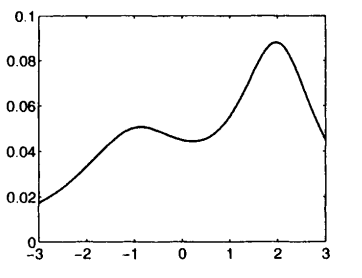
\includegraphics[max width=\textwidth]{fig31}
\caption{A graph of the function $y=$ bumpy $(x)$ of Example 3.3. }
\label{fig:fig_1_5}
\end{figure}


\textbf{EXAMPLE 3.4:} For the function bumpy $(x)$ of the previous example, find "good" approximations to the following:\\

(a) $\int_{-3}^{3} \operatorname{bumpy}(x) d x$\\

(b) The maximum and minimum values of $y=\operatorname{bumpy}(x)$ on the interval $-1.2 \leq x \leq 1$ (i.e., the height of the left peak and that of the valley) and the corresponding $x$-coordinates of where these extreme values occur.\\

(c) A solution of the equation bumpy $(x)=0.08$ on the interval $0 \leq x \leq 2$ (which can be seen to exist by examination of bumpy's graph in Figure 3.1).\\

SOLUTION: Part (a): The relevant built-in function in MATLAB for doing definite integrals is quad, which is an abbreviation for quadrature, a synonym for integration. \footnote{MATLAB has another integrator, $quad1$, that gives more accurate results for well-behaved
integrands. For most purposes, though, $quad$ is quite satisfactory and versatile as a general quadrature
tool. } The syntax is as follows:

$
\begin{array}{|l|l|}
\hline \begin{array}{l}
\text {quad('function', a, b , tol ] } \rightarrow \\
\end{array} & \begin{array}{l}
\text { Approximates the integral $\int_{a}^{n}$ function $(x) d x$ with } \\
\text {the goal of the error being less than tol.}\\
\end{array} \\
\hline
\end{array}
$\\

The function must be stored as an M-file in MATLAB's path or the exact name of a built-in function, and the name must be enclosed in 'single quotes'. \footnote{An alternative syntax (that avoids the single quotes) for this and other functions that call on M-files is $quad (@function, a, b, tol)$. Another way to create mathematical functions is to create them as so-called inline functions which are stored only in the workspace (as opposed to M-files) and get deleted when the MATLAB session is ended. Inline functions will be introduced in Chapter 6} If the whole last argument tol is omitted (along with the comma that precedes it), a maximum error goal of $10^{-3}$ is assumed. If this command is run and you just  an answer (without any additional warnings or error messages), you can safely assume that the approximation is accurate within the sought-after tolerance. 

\begin{verbatim}
>>quad ('bumpy', -3,3)  $\rightarrow$ 0.3061 
>>format long 
>> ans  -> 0.30608471060690
\end{verbatim}

As explained above, this answer should be accurate to at least three decimals. It is actually better than this since if we redo the calculation with a goal of six digits of accuracy, we obtain:


\begin{verbatim}
>> quad('bumpy',-3,3,10^(-6))
 -> 0.30608514875582
\end{verbatim}

This latter answer, which is accurate to at least six digits, agrees with the first answer (after rounding) to six digits, so the first answer is already quite accurate. There are limits to how accurate an answer we can get in this way. First of all, MATLAB works with only about 15 or so digits, so we cannot hope for an answer more accurate than this. But roundoff and other errors can occur in large-scale calculations and these can put even further restrictions on the possible accuracy, depending on the problem. We will address this issue in more detail in later depending on the problem. We will address this issue in more detail in later chapters. For many practical purposes and applications the quad function and the there will be no need to write new MATLAB M-files to perform such tasks.\\

Part (b): To (approximately) solve the calculus problem of finding the minimum value of a function on a specified interval, the relevant MATLAB built-in function is $fminbnd$ and the syntax is as follows:
\\
$
\begin{array}{|l|l|}
\hline \begin{array}{l}
\text { fminbnd('function',a,b,optimset('TolX',tol)) } \rightarrow \\
\end{array} & \begin{array}{l}
\text {Approxmiates the x-coordinate of the}\\
\text {minimum value of function(x) on}\\
\text{{[}a,b{]} with a goal of the error}\\
\text{being \textless{}tol.}
\end{array} \\
\hline
\end{array}
$\\

The usage and syntax comments for quad apply here as well. In particular, if the whole last argument optimset (' ''o1X', to1) is omlued (along whth the comma that precedes it), a maximum error goal of $10^{-3}$ is assumed. Note the syntax for changing the default tolerance goal is a bit different than for quad. This is due to the fact that fminbnd has more options and is capable of doing a lot more than we will have occasion to use it for in this text. For more information, enter help optimset.

\begin{verbatim}
>>xmin=fminbnd('bumpy',-1.2,1 ) \%We first find the x-coordinate of 
>> \% the valley  with a three digit accuracy (at least ) 
>>0.21142776202687 
>> xmin=fminbnd('bumpy',-1.2,1,optimset('TolX',le-6))  
>>\%Next let's go for 6 digits of accuracy . 
>>0.21143721018793 (=x-coordinate of valley) 

\end{verbatim}

The corresponding $y$-coordinate (height of the valley) is now gotten by evaluating bumpy $(x)$ at xmin. 

\begin{verbatim}

» ymin = bumpy (xmin) -> 0.04436776267211 (= v-coordinate of valley)

\end{verbatim}

Since we know that the $x$-coordinate is accurate to six decimals, a natural question is how accurate is the corresponding $y$-coordinate that we just obtained? One obvious thing to try would be to estimate this error by plotting bumpy $(x)$ on the interval $x \min -10^{-6} \leq x \leq x \min +10^{-6}$ and then seeing how much the $y$-coordinates vary on this plot. This maximum variation will be an upper bound for the difference of ymax and the actual value of the $y$-coordinate for the valley. When we try and plot bumpy $(x)$ on this interval as follows we get the following warning message:

\begin{verbatim}
>>x=(xmin-10^(-6)): 10^(-9):(xmin +10^(-6)) ;
>> plot(x,bumpy(x))
->Warning: Requested axes limit range too small; rendering with minimum range allowed by
machine precision.
\end{verbatim}

Also, the corresponding plot (which we do not bother reproducing) looks like that of a horizontal line, but the $y$-tick marks are all marked with the same number $(.0444)$ and similarly for the $x$-tick marks. This shows that MATLAB's plotting precision works only up to a rather small number of significant digits. Instead we can look at the vector bumpy $(x)$ with $x$ still stored as the vector above, and look at the difference of the maximum less the minimum.
\\
$
\begin{array}{|l|l|}
\hline \begin{array}{l}
\text { max(v),min(v) } \rightarrow \\
\end{array} & \begin{array}{l}
\text {For a vector v, these MATLAB commands will return the}\\
\text {maximum entry and the minimum entry; }\\
\text{ e.g.: If $v=[2  8  -50]$ then $max(v) ->$}\\
\text{ $8$, and min $(v) -> -5$.}
\end{array} \\
\hline
\end{array}
$\\

\begin{verbatim}
» max (bumpy (x) ) -min (bumpy (x)) -> 1.785377401475330e-014
\end{verbatim}

What this means is that, although $xm$ in was guaranteed only to be accurate to six decimals, the corresponding $y$-coordinate seems to be accurate to MATLAB precision, which is about 15 digits!\\

EXERCISE FOR THE READER 3.3: Explain the possibility of such a huge discrepancy between the guaranteed accuracy of xmin (to the actual $x$-value of where the bottom of the valley occurs) being $10^{-6}$ and the incredibly smaller value $10^{-14}$ of the apparent accuracy of the corresponding $ymin = bumpy(xmin)$. Make sure to use some calculus in your explanation.\\

EXERCISE FOR THE READER 3.4: Explain why the above vector argument does not necessarily guarantee that the error of $ymin$ as an approximation to the actual $y$-coordinate of the valley is less than $1.8 \times 10^{-14} \cdots$\\

We turn now to the sought-after maximum. Since there is no built-in MATLAB function (analogous to fminbnd) for finding maximums, we must make do with what we have. We can use fminbnd to locate maximums of functions as soon as we make the following observation: The maximum of a function $f(x)$ on an interval $I$, if it exists, will occur at the same $x$-value as the minimum value of the negative function $-f(x)$ on $I$. This is easy to see; just note that the graph of $y=-f(x)$ is obtained by the graph of $y=f(x)$ by turning the latter graph upside-down (more precisely, reflect it over the $x$-axis), and when a graph is turned upside-down, its peaks become valleys and its valleys become peaks. Let's initially go for six digits of accuracy:\\

\begin{verbatim}
» xmax = fminbnd (`-bumpy(x)' , -1.2 , 1, optimset('TolX',le-6))  
-> -0.86141835836638 (= x-coordinate of left peak)
\end{verbatim}


The corresponding $y$-coordinate is now:

\begin{verbatim}
>> bumpy (xmax ) -> 0.05055706241866 (= y-coordinate of left peak) 
\end{verbatim}

Part (c): One way to start would be to simultaneously graph $y=\operatorname{bumpy}(x)$ together with the constant function $y=0.08$ and continue to zoom in on the intersection point. As explained above, though, this graphical approach will limit the attainable accuracy to three or four digits. We must find the root (less than 2) of the equation bumpy $(x)=0.08$. This is equivalent to finding a zero of the standard form equation bumpy $(x)-0.08=0$. The relevant MATLAB function is fzero and its usage is as follows:\\

$
\begin{array}{|l|l|}
\hline \begin{array}{l}
\text { fzero ( function', a) } \rightarrow \\
\end{array} & \begin{array}{l}
\text {  Finds a zero of function $(x)$ near the value $x=a$ } \\
\text { (if one exists). Goal is machine precision (about 15 digits). }
\end{array} \\
\hline
\end{array}
$\\

\begin{verbatim}
>>fzero('bumpy(x)-0.08' , 1.5)
>>Zero found in the interval: [1.38,1.62].
>>1.61904252091472 (=desired solution)
>> bumpy(ans) %as a check, let's see if this value of x does what we
>>% want it to do.
-> 0.08000000000000 %Not bad!
\end{verbatim}

EXERCISE FOR THE READER 3.5: Write a function M-file with filename wiggl $\mathrm{y} \cdot \mathrm{m}$ that will store the following function:
$$
y=\sin \left(\exp \left[\frac{1}{\left(x^{2}+.5\right)^{2}}\right]\right) \sin (x) \text {. }
$$

(a) Plot this function from $x=-2$ through $x=2$.

(b) Integrate this function from $x=0$ to $x=2$ (use $10^{-5}$ as your accuracy goal).

(c) Approximate the $x$-coordinates of both the smallest positive local minimum (valley) and the smallest positive local maximum (peak)
 from $x=-2$ through $\boldsymbol{x}=2$. 
 
(d) Approximate the smallest positive solution of wiggly $(x)=x / 2$ (use $10^{-5}$ as your accuracy goal).\\


\hrule width \hsize \kern 1pt \hrule width \hsize height 0.4pt

\hspace{0.1cm}

\textbf{EXERCISES 3.2: }

\begin{enumerate}
\item (a) Create a MATLAB function M-file for the function $y=f(x)=\exp \left(\sin \left[\pi /(x+0.001)^{2}\right]\right)$ $+(x-1)^{2}$ and then plot this function on the interval $0 \leq x \leq 3$. Do it first using 10 plotting points and then using 50 plotting points and finally using 500 points.

(b) Compute the corresponding integral $\int_{1}^{3} f(x) d x$.

(c) What is the minimum value ( $y$-coordinate) of $f(x)$ on the interval $[1,10]$ ? Make sure your answer is accurate to within the nearest $1 / 10,000$th.

\item (a) Create a MATLAB function M-file for the function $y=f(x)=\frac{1}{x} \sin \left(x^{2}\right)+\frac{x^{2}}{50}$ and then plot this function on the interval $0 \leq x \leq 10$. Do it first using 200 plotting points and then using 5000 plotting points.
 
 (b) Compute the corresponding integral $\int_{1}^{10} f(x) d x$.

(c) What is the minimum value $(y$-coordinate) of $f(x)$ on the interval $[1,10]$ ? Make sure your answer is accurate to within the nearest $1 / 10,000$ th. Find also the corresponding $x$-coordinate with the same accuracy.

\item Evaluate the integral $\int_{0}^{1} \sin \left(t^{2}\right) d t$ (with an accuracy goal of $10^{-7}$ ) and compare this with the answer obtained in Example $2.7$ (Sec. 2.3).

\item (a) Find the smallest positive solution of the equation $\tan (x)=x$ using an accuracy goal of $10^{-12}$. (b) Using calculus, obtain a bound for the actual error.

\item Find all zeros of the polynomial $x^{3}+6 x^{2}-14 x+5$.

NOTE: We remind the reader about some facts on polynomials. A polynomial $p(x)$ of degree $n$ can have at most $n$ roots (that are the $x$-intercepts of the graph $y=p(x)$ ). If $x=r$ is a root and if the derivative $p^{\prime}(r)$ is not zero, then we say $x=r$ is a root of multiplicity $1 .$ If $p(r)=p^{\prime}(r)=0$ but $p^{\prime \prime}(r) \neq 0$, then we say the root $x=r$ has multiplicity 2 . In general we say $z=r$ is a root of $p(x)$ of multiplicity $a$, if all of the first $a-1$ derivatives equal zero:
$$
p(r)=p^{\prime}(r)=p^{\prime \prime}(r)=\cdots p^{(a-1)}(r)=0 \text { but } p^{(a)}(r) \neq 0
$$
Algebraically $x=r$ is a root of multiplicity a means that we can factor $p(x)$ as $(x-r)^{a} g(x)$ where $q(x)$ is a polynomial of degree $n-a$. It follows that if we add up all of the multiplicities of all of the roots of a polynomial, we get the degree of the polynomial. This information is useful in finding all roots of a polynomial.

\item Find all zeros of the polynomial $2 x^{4}-16 x^{3}-2 x^{2}+25$. For each one, attempt to ascertain its multiplicity.

\item Find all zeros of the polynomial

$$
x^{6}-\frac{25}{4} x^{3}+\frac{4369}{64} x^{4}+\frac{8325}{32} x^{3}+\frac{13655}{8} x^{2}-\frac{325}{32} x+\frac{21125}{8} .
$$

For each one, attempt to ascertain its multiplicity.

\item Find all zeros of the polynomial

$$
x^{8}+\frac{136}{5} x^{7}+210 x^{6}-\frac{165}{5} x^{5}-4094 x^{4}+\frac{4528}{5} x^{3}+17232 x^{2}+320 x+5600
$$
For each one, attempt to ascertain its multiplicity.

\item Check that the value $x=2$ is a zero of both of these polynomials:

$$
\begin{aligned}
&P(x)=x^{8}-2 x^{7}+6 x^{5}-12 x^{4}+2 x^{2}-8 \\
&Q(x)=x^{8}-8 x^{7}+28 x^{6}-61 x^{5}+95 x^{4}-112 x^{3}+136 x^{2}-176 x+112
\end{aligned}
$$

Next, use fzero to seek out this root for each polynomial using $a=1$ (as a number near the root) and with accuracy goal $10^{-12}$. Compare the outputs and try to explain why the approximation seemed to go better for one of these polynomials than for the other one.

\end{enumerate}

\end{document}